Dr. Mindy Jonas' first major discovery was the remarkable boulder game of the Fregian people. 
The Fregian kings built massive arenas with a fantastic variety of shapes and sizes. 
After surviving her own harrowing encounter with a boulder in a long-lost temple, 
Dr. Jonas found an ancient tablet describing the rules to this game.

\begin{itemize}
\item The game was played with two kinds of boulders: a white one called the fox 
  and several darker ones, called the rabbits.
\item The goal of the game was for the the fox boulder to hit the rabbit boulders 
  into the holes at the edge of the arena. Exactly one rabbit boulder
  would be hit into each hole.
\item The fox boulder could only be launched along the marked vertical, horizontal, and 
  diagonal trajectories. When it collided with a rabbit boulder, the fox boulder would 
  take the place of the rabbit and the rabbit would continue in the direction it was hit.
\item The rabbit boulders were not allowed to strike each other, and no boulder was 
  allowed to hit a sharp corner in the arena.
\item Once moving, a boulder would continue to move around the arena indefinitely, 
  bouncing off walls until it struck another boulder or sank into a hole.
\end{itemize}

I believe the August entries in Jonas's journal are records of five such arenas, and
there is a unique way to win each game. I've attached an example arena below to show
you what I mean.

Can you solve the four arenas in her journal by entering how each boulder and
hole matches up into ClueKeeper? Use the format \texttt{zB-yC-xA}, making sure to
keep the same order as the boulders are used in each puzzle. -BF

\begin{center}
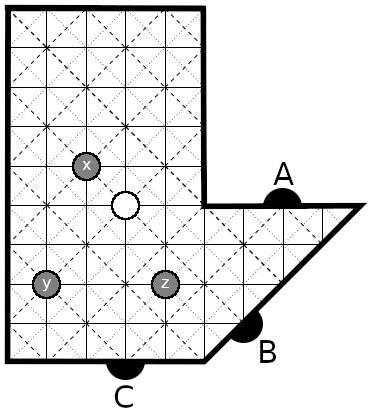
\includegraphics[width=\linewidth]{assets/Billiards_Puzzle_Tutorial.png}
\end{center}
